\documentclass[hyperref={pdfpagelabels=false}]{beamer}
% Die Hyperref Option hyperref={pdfpagelabels=false} verhindert die Warnung:
% Package hyperref Warning: Option `pdfpagelabels' is turned off
% (hyperref)                because \thepage is undefined. 
% Hyperref stopped early 
%

\usetheme{Heidelberg}
%\usetheme{iwr}

\usepackage[utf8]{inputenc}		% UTF8-Kodierung für Umlaute usw
\usepackage[T1]{fontenc} 		% Ligaturen, richtige Umlaute im PDF 
\usepackage[german,ngerman]{babel} % Silbentrennung

\setbeamercovered{invisible}

\usepackage{color}
	\definecolor{darkred}{rgb}{0.55, 0.0, 0.0}

% tikz
\usepackage{tikz}
\usepackage{varwidth}
	\usetikzlibrary{automata,positioning}
	\usetikzlibrary{shapes,arrows}
	% Define block styles
	\tikzstyle{block} = [rectangle, draw, rounded corners,text width=3.1cm] %,minimum width=20pt, minimum height=0pt]

\usepackage{amssymb,amsmath}

\usepackage{wrapfig}
\usepackage{lmodern}

\usepackage{natbib}

\usepackage{hyperref}


\newcounter{saveenumi}
\newcommand{\seti}{\setcounter{saveenumi}{\value{enumi}}}
\newcommand{\conti}{\setcounter{enumi}{\value{saveenumi}}}
% Das Paket lmodern erspart die folgenden Warnungen:
% LaTeX Font Warning: Font shape `OT1/cmss/m/n' in size <4> not available
% (Font)              size <5> substituted on input line 22.
% LaTeX Font Warning: Size substitutions with differences
% (Font)              up to 1.0pt have occurred.
%

% Wenn \titel{\ldots} \author{\ldots} erst nach \begin{document} kommen,
% kommt folgende Warnung:
% Package hyperref Warning: Option `pdfauthor' has already been used,
% (hyperref) ... 
% Daher steht es hier vor \begin{document}

\title{Constraint Programmierung für Scheduling}   
\author{Ekaterina Tikhoncheva} 
\date{08.01.2014} 

% zusaetzlich ist das usepackage{beamerthemeshadow} eingebunden 
\usepackage{beamerthemeshadow}

\begin{document}

%------------------------------------------------------------------------------%                                    Titel
\begin{frame}
\titlepage
\end{frame}
%------------------------------------------------------------------------------%                                    Plan
\begin{frame}
\frametitle{Plan}
\tableofcontents
\end{frame} 

%------------------------------------------------------------------------------%                                    CP
\section{Constraint Programmierung}
\nocite{CSP}
\nocite{CPforScheduling}
\begin{frame}

\frametitle{Was ist Constraint Programmierung?}

\begin{definition}[Constraint Programmierung]
    Die {\color{darkred} Constraint Logische Programmierung} (engl. Constraint Logic Programming) oder einfach {\color{darkred}Constraint Programmierung} (kurz {\color{darkred} \it CP}) ist ein Programmierparadigma, das unbekannte Variablen und Beziehungen zwischen ihnen durch Nebenbedingungen (Constraints) beschreibt. 
\end{definition}
\pause

{\centering
Es kam aus dem Bereich der künstlichen Intelligenz und gilt als eine Erweiterung
der Ideen der logischen Programmierung.
}

\pause
{\color{darkred}Zwei Hauptprinzipien}:
\begin{itemize}
\item Deduktion der zusätzlichen Nebenbedingungen aus den vorhandenen durch logische Folgerungen
\item Anwendung der Suchalgorithmen zum Untersuchen des Lösungsraums
\end{itemize}
\end{frame}
%                             -----------------------                         %
\begin{frame}

Constraint Programmierung:
\begin{itemize}
\centering
\item Constraint Satisfication Problem
\item Constraint Optimization Problem
\end{itemize}

\end{frame}
%                             -----------------------                         %
\subsection{Constraint Satisfication Problem}
\begin{frame}{Constraint Satisfication Problem}
  \begin{definition}
  Ein {\color{darkred} Constraint Satisfication Problem} ({\color{darkred}CSP}) ist definiert durch\begin{itemize}
	\item  die Menge $X= \{ x_1,x_2,\dots, x_n\}$ diskrete Variablen zusammen mit ihren endlichen Definitionsbereichen $\{ D_1,D_2,,\dots D_n\}$ 
	\item die Menge der Bedingungen $C_{ijk\dots}$ zwischen den Variablen $x_i, x_j, x_k, \dots$, die die möglichen Werte der Variablen zusätzlich einschränken.
  \end{itemize}
  Ein CSP besitzt eine {\bf (zulässige) Lösung}, wenn eine Zuweisung der Werten aus den  Definitionsbereichen zu jeder Variable existiert, sodass alle Bedingungen erfüllt sind.
  \end{definition}
\end{frame}
%                             -----------------------                         %
\begin{frame}
Die Variablen können von verschiedenen Typen sein:\\ ganzzahlig, boolean, symbolisch, Mengen.
\vspace{15pt}

Dafür gibt es verschiedene Typen der Bedingungen:
\begin{itemize}
	\setlength{\itemsep}{0pt}
	\item mathematische (Fertigstellungszeit = Startzeit + Bearbeitungszeit),
	\item disjunktive (Jobs $J_1$ und $J_2$ müssen an verschiedenen Maschinen abgearbeitet werden),
	\item relational (die Maschine $I$ kann höchstens vier Jobs abarbeiten),
	\item explizite (die Arbeiten $J_1$, $J_2$ und $J_5$ können nur auf der Maschine $1$ abgearbeitet werden).
\end{itemize}
\end{frame}
%                             -----------------------                         %
%                          Algprithmus
\begin{frame}{Lösung des Constraint Satisfaction Problems}

\centering
 \begin{tikzpicture}[overlay]
     \node at ( 0,-0.5) (picture) {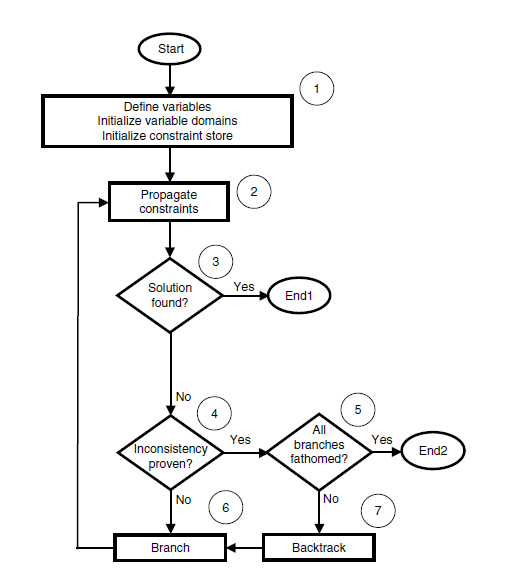
\includegraphics[scale = 0.45]{fig/CSPalgorithm.png}};
     \node [block, text width=2.5cm] at (4, 0.5)(comment1)
     {
     	\tiny 1: Initialisiere das Modell
     };
  \end{tikzpicture}
\end{frame}
%
\begin{frame}{Lösung des Constraint Satisfaction Problems}
\centering
 \begin{tikzpicture}[overlay]
     \node at ( 0,-0.5) (picture) {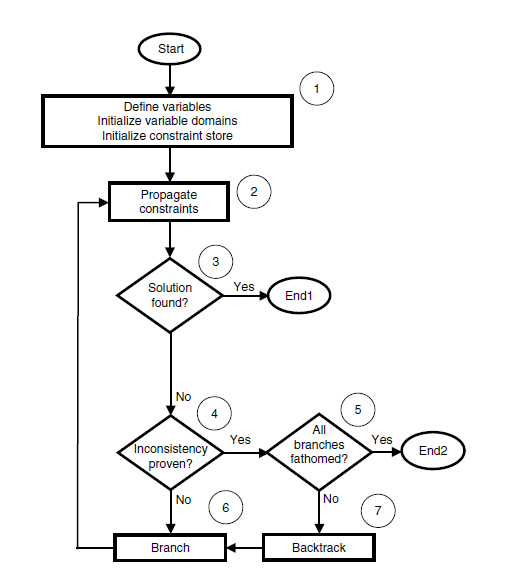
\includegraphics[scale = 0.45]{fig/CSPalgorithm.png}};
     \node [block] at (4, 0.5)(comment1) 
     {
     	\tiny 2: {\bf Bedingungsfortpflanzung}\\
     	prüft die Widerspruchsfreiheit \\ der im Problem
     	vorhandenen \\ Bedingungen, um die neuen \\ Bedingungen ableiten zu \\ können \\ (eng. {\color{darkred}arc consistency 
     	checking}) \\
     };
     
     \pause
     
     \node [block, color=red, text width=0.8cm] at (-3, 0.5)(comment2)
     {
     	\tiny {\color{darkred}}Beispiel
     };
  \end{tikzpicture}
\end{frame}
%
\begin{frame}{Lösung des Constraint Satisfaction Problems}
\centering
 \begin{tikzpicture}[overlay]
     \node at ( 0,-0.5) (picture) {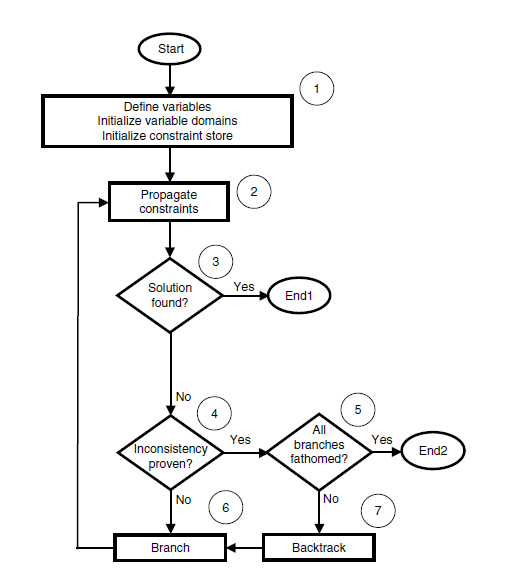
\includegraphics[scale = 0.45]{fig/CSPalgorithm.png}};
     \node [block] at (4, 0.5)(comment1)
     {
     	\tiny 3: Falls eine Lösung des \\ Problems gefunden ist, terminiert der Algorithmus \\
     };
  \end{tikzpicture}
\end{frame}
%
\begin{frame}{Lösung des Constraint Satisfaction Problems}
\centering
 \begin{tikzpicture}[overlay]
     \node at ( 0,-0.5) (picture) {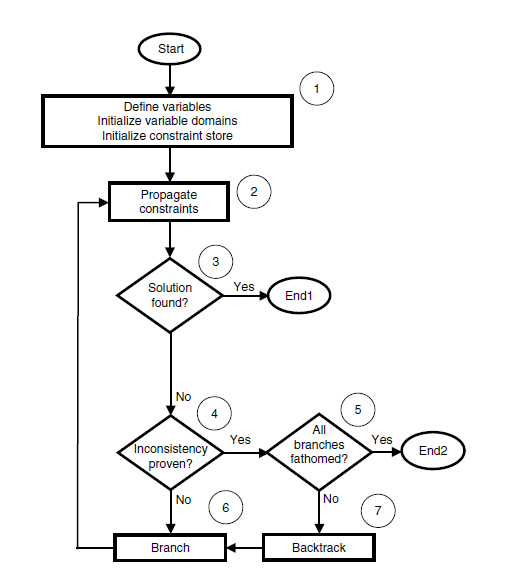
\includegraphics[scale = 0.45]{fig/CSPalgorithm.png}};
     \node [block, text width=3.7cm] at (4, 0.5)(comment1)
     {
     	\tiny 4: Ist das Problem widersprüchlich?\\
     };
  \end{tikzpicture}

\end{frame}
%
\subsection{Lösung des Constraint Satisfaction Problems}
\begin{frame}{Lösung des Constraint Satisfaction Problems}
\centering
 \begin{tikzpicture}[overlay]
     \node at ( 0,-0.5) (picture) {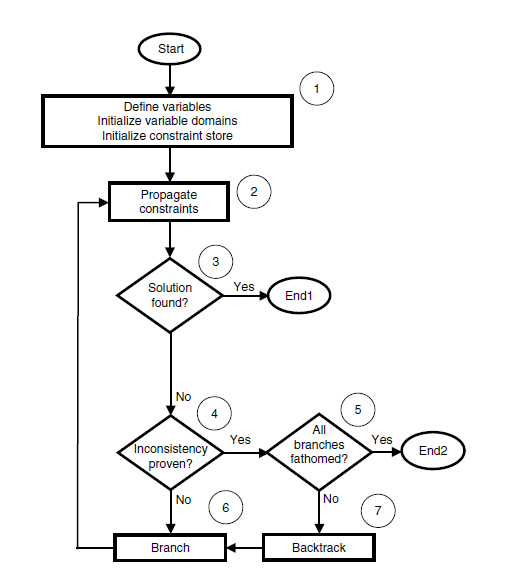
\includegraphics[scale = 0.45]{fig/CSPalgorithm.png}};
     \node [block, text width=3.7cm] at (4, 0.5)(comment1) 
     {
     	\tiny 5: Sind alle Teilprobleme untersucht? Falls ja, dann ist das ursprüngliche Problem widersprüchlich und der Algorithmus terminiert.\\
     };
  \end{tikzpicture}
\end{frame}

%
\begin{frame}{Lösung des Constraint Satisfaction Problems}
\centering
 \begin{tikzpicture}[overlay]
     \node at ( 0,-0.5) (picture) {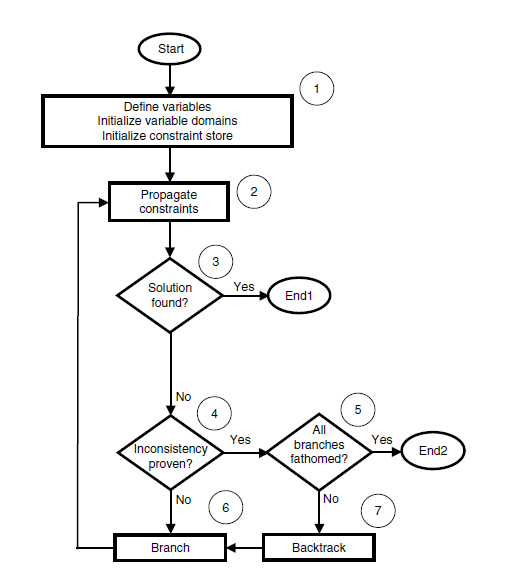
\includegraphics[scale = 0.45]{fig/CSPalgorithm.png}};
     \node [block,text width=3.7cm] at (4, 0.5)(comment1) {\tiny 6:
     	{\bf Branching}\\ Teile das ursprüngliche Problems in eine Menge von Teilproblemen $\rightsquigarrow$  Entscheidungsbaum\\};
     
     \pause
     
     \node [block, text width=3.5cm] at (-4.5, 0.5)(comment2)
     {
        \tiny oft\qquad {\color{darkred} das Backtracking-Verfahren} \\
     	\qquad $'-'$ ineffizient \\
     	Alternativ\qquad {\color{darkred}lookahead Verfahren} 
     	\qquad(z.B. Forward checking, MAC) \\
     };
     
     \pause
     
     \node [block, color = red, text width=3.5cm] at (-4.5, -1.0)(comment3)
     {
     	\tiny \color{black}{\bf ?}: wo wird als erstes verzweigt\\
     	Z.B in die Variable mit dem kleinsten Definitionsbereich \\
     };
     
     \pause
     
     \node [block, color = red, text width=3.5cm] at (-4.5, -2.5)(comment4)
     {
     	\tiny \color{black}{\bf ?}:welchen Wert soll die verzweigte Variable annehmen\\
     	Z.B den kleinsten Wert aus dem Definitionsbereich \\
     };
  \end{tikzpicture}
\end{frame}
%
\begin{frame}{Lösung des Constraint Satisfaction Problems}
\centering
 \begin{tikzpicture}[overlay]
     \node at ( 0,-0.5) (picture) {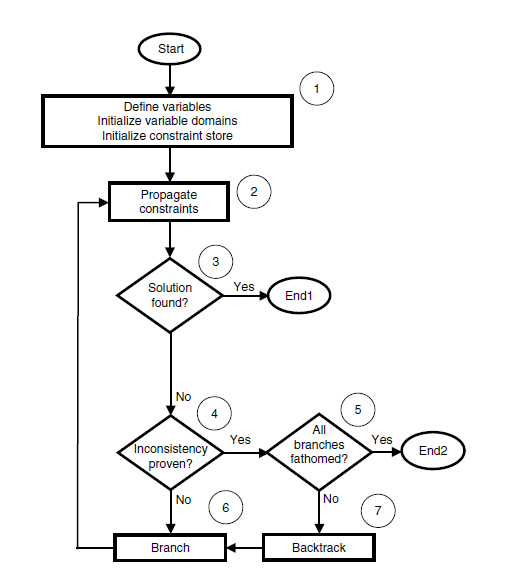
\includegraphics[scale = 0.45]{fig/CSPalgorithm.png}};
     \node [block] at (4, 0.5)(comment1) 
     {
     	\tiny 7: Wähle nächstes Teilproblem und versuch es zu lösen \\
     };
  \end{tikzpicture}
\end{frame}
%                             -----------------------                         %
%                          Constraint Optimization Problem                    %
\subsection{Constraint Optimization Problem}
\begin{frame}{Constraint Optimization Problem}

	{\color{darkred} Constraint Optimization Problem} ({\color{darkred}COP}) kann einfach aus dem CSP erweitert werden:
	\begin{itemize}
	\item Angenommen unser COP hat eine Zielfunktion Z, die minimiert werden soll. 
	
	\item Ohne $Z$ habe wir ein CSP und seine Lösung können wir
	mit Hilfe des Algorithmus finden.
	
	\item Sobald eine Lösung von CSP
	gefunden wurde, berechne den Wert der Zielfunktion Z0 und füge die Bedingung Z < Z0 zum Problem hinzu 
	
	\item Löse neues CSP und so weiter, bis es zu einem Widerspruch gekommen ist und alle Zweige
	im Suchbaum untersucht wurden.
	\item Die zuletzt gefundene zulässige Lösung ist somit die Lösung des COP.
	\end{itemize}
\end{frame}
%                             -----------------------                         %
%                    Vorteil des Constraint Programmierung                    %
\subsection{Vorteil des Constraint Programmierung}
\begin{frame}{Vorteil des Constraint Programmierung}
\begin{itemize}
	\vspace{30pt}
	\item Analog zu den Programmiersprachen ist die Benutzung einer Variablen als Indizes von anderen Variablen erlaubt\\
	$\rightsquigarrow$ Reduktion der Anzahl der Entscheidungsvariablen
	
	\vspace{30pt}
	Z.B. Berechnung der Kosten einer Jobreihenfolge
	
	\vspace{10pt}
	\begin{tikzpicture}
		\node [block, text width=5.1cm] at (2, 0.5)(IP) 
		{
			\tiny {\color{darkred} IP:} $n(n-1)$ Variablen \\
			$y[i,j]\in \{0,1\}$ 
					$1$, falls Job $i$ ein direkter Vorgänger des Jobs $j$ ist\\
			\vspace{3pt}
			Gesamte Preis der Jobreihenfolge : $\sum_{i,j,i\not =  j} {cost[i,j]y[i,j]}$ \qquad\qquad {\color{red} }\\
		};

		\node [block,text width=5.cm] at (7.5, 0.5)(CP) 
		{
			\tiny {\color{darkred} CP:} n Variablen \\
			$job[k]=$ Index des k-ten Jobs in Reihenfolge \\
			\vspace{5pt}
			Gesamte Preis der Jobreihenfolge : $\sum_{k>1} {cost[job[k-1],job[k]]}$ \qquad\qquad {\color{red} }\\
		};
	\end{tikzpicture}
	\end{itemize}
\end{frame}
%                             -----------------------                         %
\begin{frame}

	\begin{itemize}
	
	\item Einfachere Notation der Nebenbedienungen
	
	\vspace{5pt}
	{\tiny
	Angenommen wir haben ein Problem mit zwei Maschinen. Die Variablen $MaschineA$ und $MaschineB$ können den Wert $0$ haben, falls es keinen Job gibt, der auf der Maschine abgearbeitet werden muss, oder $1$ ansonsten. Wir suchen nach einer solchen Zuordnung der Jobs zu diesen Maschinen, so dass nur eine Maschine in Betrieb sein kann.\\
	}
	\vspace{5pt}
	\begin{tikzpicture}
		\node [block, text width=5.1cm] at (2, 0.5)(IP) 
		{
			\tiny {\color{darkred} IP:} $MaschineA+MaschineB = 1$  \\
		};

		\node [block,text width=5.cm] at (7.5, 0.5)(CP) 
		{
			\tiny {\color{darkred} CP:} $MaschineA\not =MaschineB$\\
		};
	\end{tikzpicture}
	
	\vspace{5pt}

	{\tiny
	Seien die Variablen $MaschineA$ und $MaschineB$ ganzzahlig und ihre Werte sind die Nummern der Jobs, die auf diesen Maschinen abgearbeitet werden.
	
	Die Bedingung lautet \glqq ein Job kann nicht auf zwei Maschinen abgearbeitet werden\grqq.\\}
	
	\vspace{5pt}
	\begin{tikzpicture}
		\node [block, text width=5.1cm] at (2, 0.5)(IP) 
		{
			\tiny {\color{darkred} IP:}\\ 
			$(MaschineA - MaschineB - \epsilon +\sigma BigM \ge 0)$ \\
			$(MaschineB - MaschineA - \epsilon +(1-\sigma) BigM \ge 0)$ \\
			 $\sigma\in{0,1}$  \\
		};

		\node [block,text width=5.cm] at (7.5, 0.5)(CP) 
		{
			\tiny {\color{darkred} CP:}\\
			$MaschineA\not =MaschineB$\\
		};
	\end{tikzpicture}
	
	\vspace{5pt}
	{\tiny 
	Die Fertigstellungszeit-Bedingung: falls Job $A$ und Job $B$ auf einer Maschine abgearbeitet werden, dann muss die Bearbeitung von Job $A$ früher fertig werden, als die Bearbeitung vom Job $B$ beginnt, oder umgekehrt.\\}

	\vspace{5pt}
	\begin{tikzpicture}
		\node [block, text width=5.1cm] at (2, 0.5)(IP) 
		{
			\tiny {\color{darkred} IP:}\\ 
			$(A.start - B.end - \epsilon +\sigma BigM \ge 0)$ \\
			$(B.start - A.end- \epsilon +(1-\sigma) BigM \ge 0)$ \\
			$\sigma\in{0,1}$  \\
		};

		\node [block,text width=5.cm] at (7.5, 0.5)(CP) 
		{
			\tiny {\color{darkred} CP:}\\
			$(A.start > B.end) Xor (B.start > A.end)$\\
		};
	\end{tikzpicture}
\end{itemize}

\end{frame}
%                             -----------------------                         %
\begin{frame}
Allgemein gilt:

\vspace{30pt}
\begin{tikzpicture}
	\node [block, text width=5.1cm] at (2, 0.5)(IP) 
	{
		\small {\color{darkred} IP:}\\ 
		\begin{itemize}
		 \item wichtig ist mathematische Struktur des Problems
		 \item zentrale Rolle spielt Zielfunktion 
		 \item gesucht wird die kleinste Menge der Nebenbedingungen, die ausreichend ist, den Kernpunkt des Problems zu beschreiben
		 \end{itemize}
	};
	\node [block,text width=5.cm] at (7.5, 0.5)(CP) 
	{
		\small {\color{darkred} CP:}\\
		\begin{itemize}
		 \item lässt großen Spielraum im Entwerfen von Nebenbedingungen und Suchalgorithmen
		 \item konzentriert sich auf Nebenbedingen 
		 \item soviel Nebenbedingungen, wie möglich
		 \end{itemize}
	};
	\end{tikzpicture}
\end{frame}

%------------------------------------------------------------------------------%
%                       Beispiele aus der Scheduling Theorie
\section{Beispiele aus der Scheduling Theorie}
%                             -----------------------                         %
\subsection{Minimieren der gewichteten Gesamtverspätung}
\begin{frame}[allowframebreaks]{$1||\sum{w_jT_j}$}

Es ist ein bekanntes {\color{darkred}$NP$-hartes Problem}. 

\begin{block}{}
Es gibt einen Lösungsansatz mittels {\color{darkred}Dynamischer Programmierung}, der einen pseudopolynomialen Algorithmus liefert.
\end{block}
\vspace{10pt}
Die einfachste Formulierung des Problems in CP:
\begin{itemize}
\item $n$ Variablen $s_j$ mit dem Definitionsbereich $[0\dots \sum_{j=1..n}p_j]$ für Startzeiten
\item $n$ Variablen $C_j$ mit dem Definitionsbereich $[0\dots \sum_{j=1..n}p_j]$ für die Fertigstellungszeiten von Jobs.
\end{itemize}

\vspace{20pt}

\begin{block}{CP-Formulierung}
\begin{align}
 \min & \sum_{j}{w_jT_j} \nonumber \\
 s.t.\quad C_j & = p_j + s_j\qquad\qquad \forall j=1..n \nonumber \\
 C_j  & \le s_k \vee  C_k \le s_j \qquad \forall j,k=1..n,\ k>j \nonumber
\end{align}
\end{block}

Insgesamt: $2n$ Variablen und $\frac{n(n+1)}{2}$ Nebenbedingungen.

\newpage

Eine andere Formulierung ist möglich:
\begin{itemize}
\item ersetze $n$ Variablen $s$ durch $n$ Variablen $pos$ mit den Definitionsbereichen $[1..n]$, wobei $pos[j]$ die Position des Jobs $j$ in der Bearbeitungsreihenfolge ist.
\end{itemize}
\begin{block}{} \begin{align}
	pos_j & \not= pos_k\qquad\qquad \forall j,k=1..n,\ k>j \nonumber \\
	pos_j  & > pos_k \Leftrightarrow  C_j \ge C_k + p_j \qquad \forall j,k=1..n,\ k\not=j \nonumber \\
	pos_j  & = 1 \Rightarrow C_j=p_j \qquad \forall j=1..n \nonumber
\end{align} \end{block}
Insgesamt: $2n$ Variablen und $\frac{3n^2-n}{2}$ Nebenbedingungen, aber die Optimierung ist viel langsamer

\newpage
{\small
Weitere Bedingungen:

\vspace{10pt}
 Wird ein Job auf der Position $j$ platziert, ist die untere Schranke seiner Fertigstellungszeit gleich der Summe seiner Bearbeitungszeit und der Summe $p_i$ von $j-1$ Jobs mit den kleinsten Bearbeitungszeiten.
\begin{block}{}
\begin{align}
  pos_j=k \wedge j<=k  & \Rightarrow C_j \ge \sum_{l<=k} p_l \nonumber \\
  pos_j=k \wedge j>k  & \Rightarrow C_j \ge p_j+\sum_{l<k} p_l \nonumber 
\end{align}
\end{block}
\vspace{8pt}
Mögliche Heuristik für das Suchverfahren WMDD (\glqq {\it weighted modified due date} \grqq)
}
\end{frame}
%                             -----------------------                         %
%                              Job Shop Scheduling                            %
\subsection{Job Shop Scheduling}
\begin{frame}[allowframebreaks]{$Jm||C_{max}$}
\nocite{CSP}
\small 

\vspace{40pt}
\begin{block}{}
Die Aufgabe ist $n$ Jobs zu $m$ Maschinen zuordnen, wobei jeder Job $j$ aus einer Menge von Operationen $O_j$ besteht, die in einer bestimmten Reihenfolge abgearbeitet werden müssen.
\end{block}

\begin{block}{}
Zur Modellierung dieses Problems verwendet man so genannte {\color{darkred}disjunktive Graphen} und
zur Lösung das {\color{darkred}Branch \& Bound} Verfahren.
\end{block}

\newpage

CP-Formulierung:
\begin{itemize}
\item definiere eine Variable $s_o$ für die Startzeit der Operation $o\in O_j$, $s_o\in \{0,1,\dots C\}$, wobei $C_{max}<C$ ist. 
\item Oder besser :  $s_o\in[\sum_{o'\in pred(o)}p_{o'}\dots\ C-p_o-\sum_{o'\in succ(o)}p_{o'}]$, wobei $pred(o)$ der Vorgänger und $succ(o)$ ein Nachfolger von einer Operation $o$ sind.
\end{itemize}

\begin{block}{Die Nebenbedingungen} \begin{align}
  s_o + p_o \le s_{o'} &\qquad  o,o'\in O_j,\ o'\in succ(o),\ j=1\dots n \nonumber \\
  s_o + p_o \le C &\qquad  o\in O \nonumber \\
  s_o + p_o \le s_{o'}\ & \vee\ s_{o'} + p_{o'} \le s_{o} \qquad o,o'\in O, o\not=o', m_o=m_{o'} \nonumber 
\end{align}
\end{block}
wobei $O$ die Menge aller Operationen bezeichnet.


\newpage

Wie kann man die Bedingungsfortpflanzung für dieses Modell effektiv durchführen? 

Definiere für jede $o$ 
\begin{itemize}
\item die frühst möglichste Startzeit $est(o)$
\item die spät möglichste Startzeit $lst(o)$
\end{itemize}

Aus {\color{blue}$s_o + p_o \le s_{o'}$} folgt {\color{darkred}$s_o+p_0\le lst(o')$} und {\color{darkred}$est(o)+p_o\le p_{o'}$}

$\Rightarrow$ lösche die Werte größer als {\color{red}$lst(o')-p_o$} und kleiner als {\color{red}$est(o)+p_o$} aus den Definitionsbereichen von $s_o$ und $s_{o'}$.

\vspace{5pt}
Aus  {\color{blue}$(s_o + p_o \le s_{o'})\vee(s_{o'} + p_{o'} \le s_{o})$} folgt\\ \qquad \qquad
{\color{darkred} $(s_o\le lst(o') - p_o)\vee(s_o \ge est(o') + p_{o'})$}

$\Rightarrow$ falls $lst(o') - p_o + 1 \le est(o') + p_{o'} -1$ gilt, lösche {\color{red} $[lst(o') - p_o + 1 \dots est(o') + p_{o'} -1]$} aus dem Definitionsbereich von $s_o$.

\end{frame}
%                             -----------------------                         %
%                                 Timetabling                                 %
\subsection{Timetabling}
\begin{frame}[allowframebreaks]{Timetabling}
\nocite{Timetabling}
\small

\begin{block}{Aufgabe}
Einen Spielplan für $9$ Basketball-Teams erstellen. Es sollen $18$ Termine festgelegt werden, sodass an jedem Termin $8$ Teams spielen und ein Team nicht spielt (d.h. hat \glqq bye\grqq). Alle Termine sollten in neun Wochen mit einem Wochenende und einen Arbeitstag pro Woche geplant werden.
\end{block}

\newpage

Das Problem wird in drei Phasen gelöst: \begin{itemize}
\setlength{\itemsep}{0pt}
\item Generierung von einem Muster (engl. pattern) für jedes Team, das für jeden Termin feststellt, ob Team ein Heim-, Auswärtsspiel oder \glqq bye\grqq\ spielen kann. 
\item Suche nach einer Menge von $9$ Mustern, die die Erstellung eines Zeitplanes ermöglichen.
\item Generierung eines Zeitplans, indem man anhand der Menge von Mustern die Zuordnung von Spielen zu den Teams und Paare von Gegner bestimmt.
\end{itemize}

\newpage

\begin{block}{Phase $1$: Pattern-Generierung (CSP)}
Binäre Variablen $h_j, a_j, b_j, j=1\dots 18,$ für Heimspiele, Auswärtsspiele und byes 
\begin{itemize}
\setlength{\itemsep}{0pt}
\item jedes Team hat nur ein Spiel an jedem Termin: $h_j+a_j+b_j = 1$

\item s.g. Mirroring: Termine sind paarweise in die vorgegebene Menge $m$ gruppiert, jedes Paar bezeichnet Spiele der gleichen Teams: $h_j=a_{j'},\ a_j=h_{j'},\ b_j=b_{j'}\ (j, j')\in m$

\item die beiden letzten Spielen können nicht beide Auswärtsspiele sein : $a_{17}+a_{18} = 2$

\item Es sind nicht mehr als zwei Auswärtsspiele nacheinander erlaubt:\\ $a_j+a_{j+1}+a_{j+2}<3$ 

\item Es sind nicht mehr als zwei Heimspiele nacheinander erlaubt:\\ $h_{j}+h_{j+1}+h_{j+2}<3$ 
\end{itemize}
\end{block}

\newpage

\begin{block}{}
\begin{itemize}
\item Es sind nicht mehr als drei Auswärtsspiele oder byes  nacheinander erlaubt: \\
$a_j+b_j+a_{j+1}+b_{j+1}+a_{j+2}+b_{j+2}+a_{j+3}+b_{j+3}<4$ 

\item Es sind nicht mehr als vier Heimspiele oder byes nacheinander erlaubt:\\
$h_j+b_j+h_{j+1}+b_{j+1}+h_{j+2}+b_{j+2} +h_{j+3} ++b_{j+3} +h_{j+4}+b_{j+4} <5 $

\item An allen Wochenenden spielt jedes Team vier Heim-, vier Auswärtsspiele und ein bye:   $\sum_{j\in\{2,4,\dots 18\}}h_j = 4$, $\sum_{j\in\{2,4,\dots 18\}}a_j = 4$, $\sum_{j\in\{2,4,\dots 18\}}b_j = 1$

\item Jedes Team spielt ein Heimspiel oder bye mindestens an zwei der ersten fünf Wochenenden $\sum_{j\in\{2,4,6,8,10\}}(h_j+b_j) \ge 2$
\end{itemize}
\end{block}

Die effektivste Suchstrategie in diesem Fall ist das Durchzählen der möglichen Werte vom $h,a,b$ in der Reihenfolge $h_1,a_1,b_1,h_2,a_2\dots$.


\begin{block}{Phase $2$:  Menge von Mustern (CSP)}

\begin{align}
  \sum_{i}x_i=9 &  \nonumber \\
  \sum_{i}h_{ij}x_i = 4,\ \sum_{i}s_{ij}x_i = 4, &\ \sum_{i}b_{ij}x_i = 1 \qquad  j=1\dots 18 \nonumber \\
  x_i+x_{i'} <1  &\qquad  j=1\dots 18,\ i,i'=1\dots 9,\ i\not=i', \nonumber\\
  & (h_{ij}=0 \vee a_{i'j}=0)\wedge(a_{ij}=0 \vee h_{i'j}=0) \nonumber  
\end{align}
\end{block}

\newpage

\begin{block}{Phase $3$: Erstellung von einem zulässigen Zeitplan}
Ordne erst jedes Team zu einem von $9$ vorhandenen Mustern zu und danach sucht es für jedes Team nach den möglichen Gegnern an jedem Termin.

\begin{itemize}
\item formuliere die Aufgabe als ein CP Modell, das jeweils für jedes Team und jeden Termin einen Gegner und eine Spielart (Heim-/Auswärtsspiel oder bye) berechnet
\item Die Nebenbedingungen werden von allgemeinen Bedingungen an ein Rundenturnier und Bedingungen aus Phase $1$ bestimmt.
\end{itemize}
\end{block}

\end{frame}

%------------------------------------------------------------------------------%                                    References
\begin{frame}[allowframebreaks]
	\frametitle{References}
	\bibliographystyle{plain}
	\bibliography{bibliographie}
\end{frame}

%                                    ------------                                            %
\begin{frame}{The End}
\centering
\LARGE
\color{red}
 Vielen Dank für Ihre Aufmerksamkeit!
 \nocite{BeamerTheme}
\end{frame}

\begin{frame}
\centering
\begin{figure}
	
\includegraphics{who.png}
\end{figure}
\end{frame}
\end{document}
